\documentclass{beamer}
\usepackage[utf8]{inputenc}

\usetheme{Madrid}
\usecolortheme{default}
\usepackage{amsmath,amssymb,amsfonts,amsthm}
\usepackage{txfonts}
\usepackage{tkz-euclide}
\usepackage{listings}
\usepackage{adjustbox}
\usepackage{array}
\usepackage{tabularx}
\usepackage{gvv}
\usepackage{lmodern}
\usepackage{circuitikz}
\usepackage{tikz}
\usepackage{graphicx}

\setbeamertemplate{page number in head/foot}[totalframenumber]

\usepackage{tcolorbox}
\tcbuselibrary{minted,breakable,xparse,skins}



\definecolor{bg}{gray}{0.95}
\DeclareTCBListing{mintedbox}{O{}m!O{}}{%
  breakable=true,
  listing engine=minted,
  listing only,
  minted language=#2,
  minted style=default,
  minted options={%
    linenos,
    gobble=0,
    breaklines=true,
    breakafter=,,
    fontsize=\small,
    numbersep=8pt,
    #1},
  boxsep=0pt,
  left skip=0pt,
  right skip=0pt,
  left=25pt,
  right=0pt,
  top=3pt,
  bottom=3pt,
  arc=5pt,
  leftrule=0pt,
  rightrule=0pt,
  bottomrule=2pt,
  toprule=2pt,
  colback=bg,
  colframe=orange!70,
  enhanced,
  overlay={%
    \begin{tcbclipinterior}
    \fill[orange!20!white] (frame.south west) rectangle ([xshift=20pt]frame.north west);
    \end{tcbclipinterior}},
  #3,
}
\lstset{
    language=C,
    basicstyle=\ttfamily\small,
    keywordstyle=\color{blue},
    stringstyle=\color{orange},
    commentstyle=\color{green!60!black},
    numbers=left,
    numberstyle=\tiny\color{gray},
    breaklines=true,
    showstringspaces=false,
}
\title 
{MatGeo Assignment 1.2.13}

\author
{AI25BTECH11007}
\begin{document}

\frame{\titlepage}
\begin{frame}{Question}
If (1, 2), (4, y), (x, 6) and (3, 5) are the vertices of a parallelogram taken in order, find
x and y.\\
\end{frame}
\begin{frame}{Theoretical Solution}
\noindent
Let us solve the given equation theoretically and then verify the solution computationally \\
According to the question, \\

We are given the vertices of a parallelogram in order:
$$A(1,2), \; B(4,y), \; C(x,6), \; D(3,5).$$
\end{frame}

\begin{frame}{Property}
\textbf{In a parallelogram, the diagonals bisect each other.So, the midpoints of the diagonals are equal.}
\end{frame}
\begin{frame}{Theoretical Solution}

\text{Given the vertices of a parallelogram: } 
$$A(1,2), \; B(4,y), \; C(x,6), \; D(3,5).$$

\text{Property: In a parallelogram, diagonals bisect each other.}
\text{Midpoint of } AC = \text{Midpoint of } BD

\begin{equation}
\frac{1}{2}
\myvec{
1 + x \\
2 + 6
}
=
\frac{1}{2}
\myvec{
4 + 3 \\
y + 5
}
\end{equation}

\begin{equation}
\myvec{
\frac{1+x}{2} \\
\frac{8}{2}
}
=
\myvec{
\frac{7}{2} \\
\frac{y+5}{2}
}
\end{equation}

\begin{equation}
\frac{1+x}{2} = \frac{7}{2}, 
\quad 
\frac{8}{2} = \frac{y+5}{2}
\end{equation}

\begin{equation}
x = 6, 
\quad 
y = 3
\end{equation}

\begin{equation}
\therefore \; x=6, \; y=3
\end{equation}
\end{frame}


\begin{frame}{Plot}
    \centering
    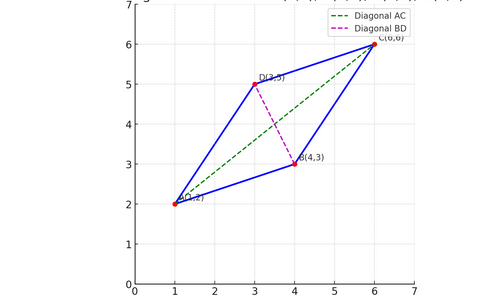
\includegraphics[width=\columnwidth, height=0.8\textheight, keepaspectratio]{figs/fig1.png} 
    \label{The visual of the parallelogram with vertices labeled and diagonals shown}
\end{frame}

\begin{frame}{Conclusion}
    

From the figure it is clearly verified that theoritical solution matches with the computational solution.
\end{frame}
\end{document}